%---------------------------------------------------------------------------------------------------
% GAME LOGIC
%---------------------------------------------------------------------------------------------------
\subsection{Aperçu globale}

Ce que nous appelons système est en réalité une assemblage de plusieurs logicielles qui communiquent entre eux :

\begin{figure}[H] 
\centering
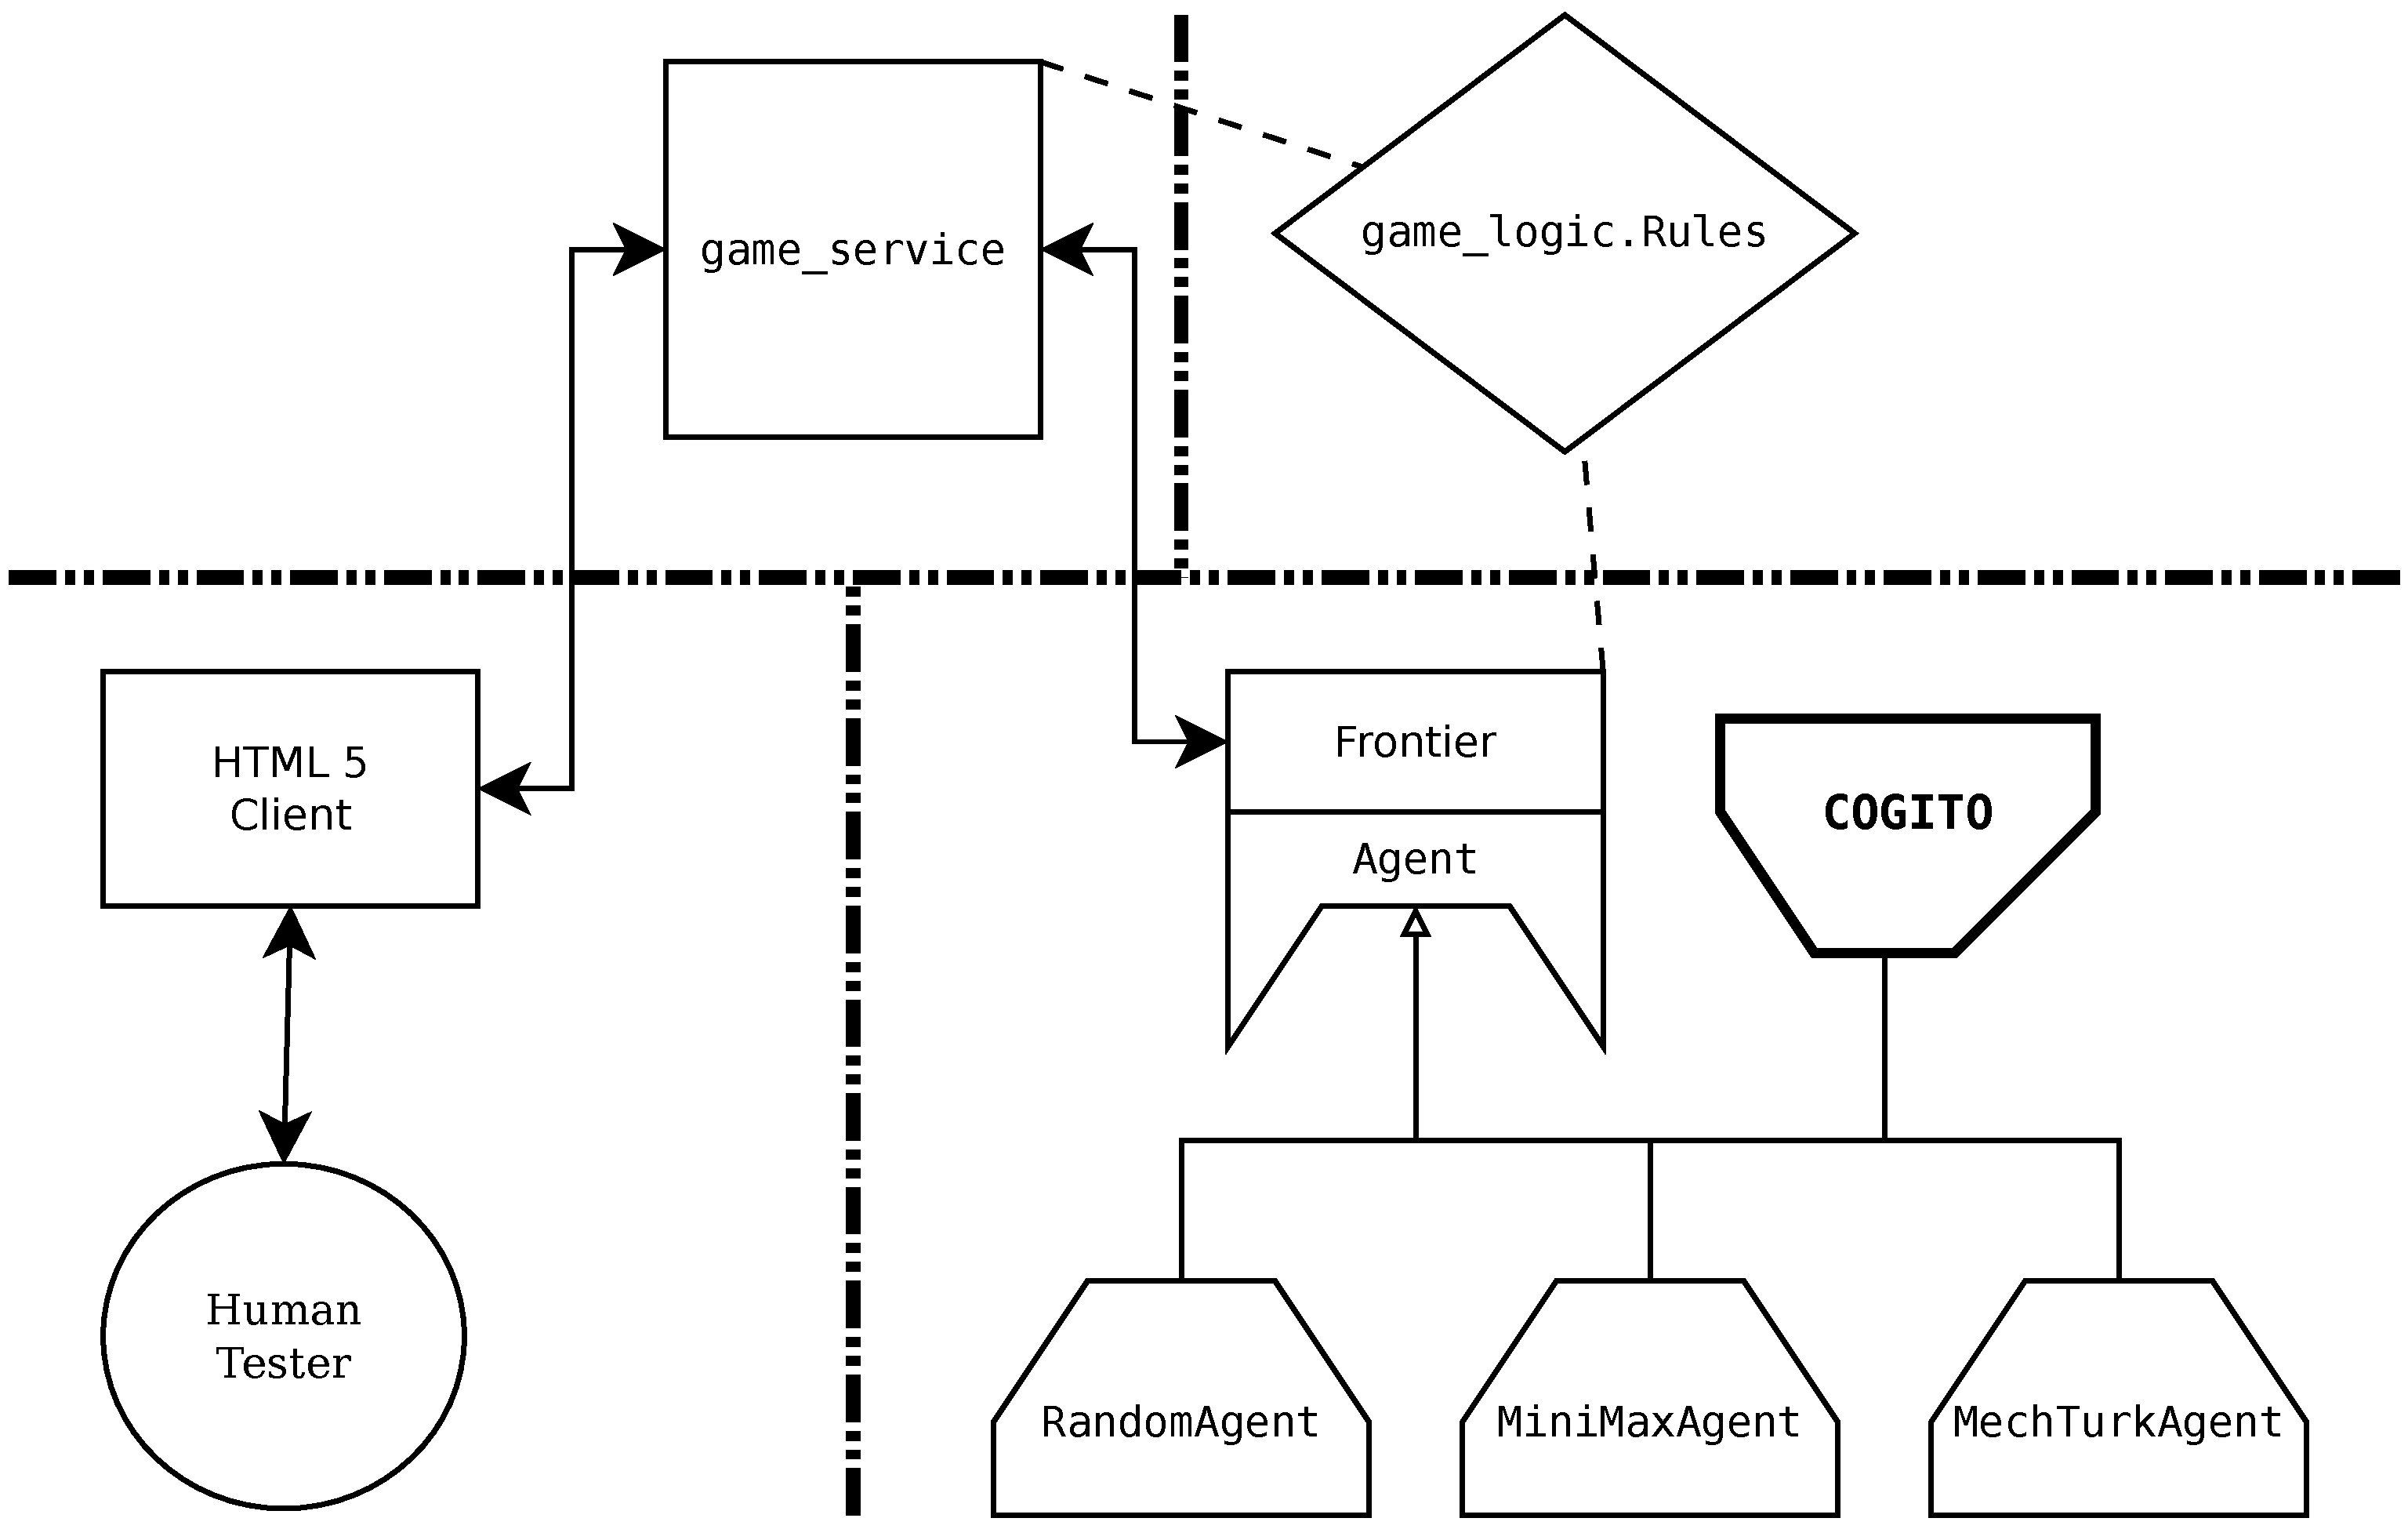
\includegraphics[width=\textwidth]{files/william/archi_full} 
\caption{Aperçu global du système.} 
\end{figure}

Avant de se concentrer sur la \cogito{} lui même nous expliquerons rapidement l'implémentation de l'infrastructure de test, que nous pouvons voir comme l'environnement.

\subsection{Bibliothèque \texttt{\gls{game_logic}}}

Dans le chapitre~\ref{subsection_architecture_generale} nous avons introduit le module conceptuel \emph{Rule Book}, qui génère un ensemble coups possibles, chacun associé à son plateau résultant. Pour ce faire ce module doit pouvoir décider de la légalité d'un coup et connaître ses conséquences. 

\begin{figure}[H] 
\centering
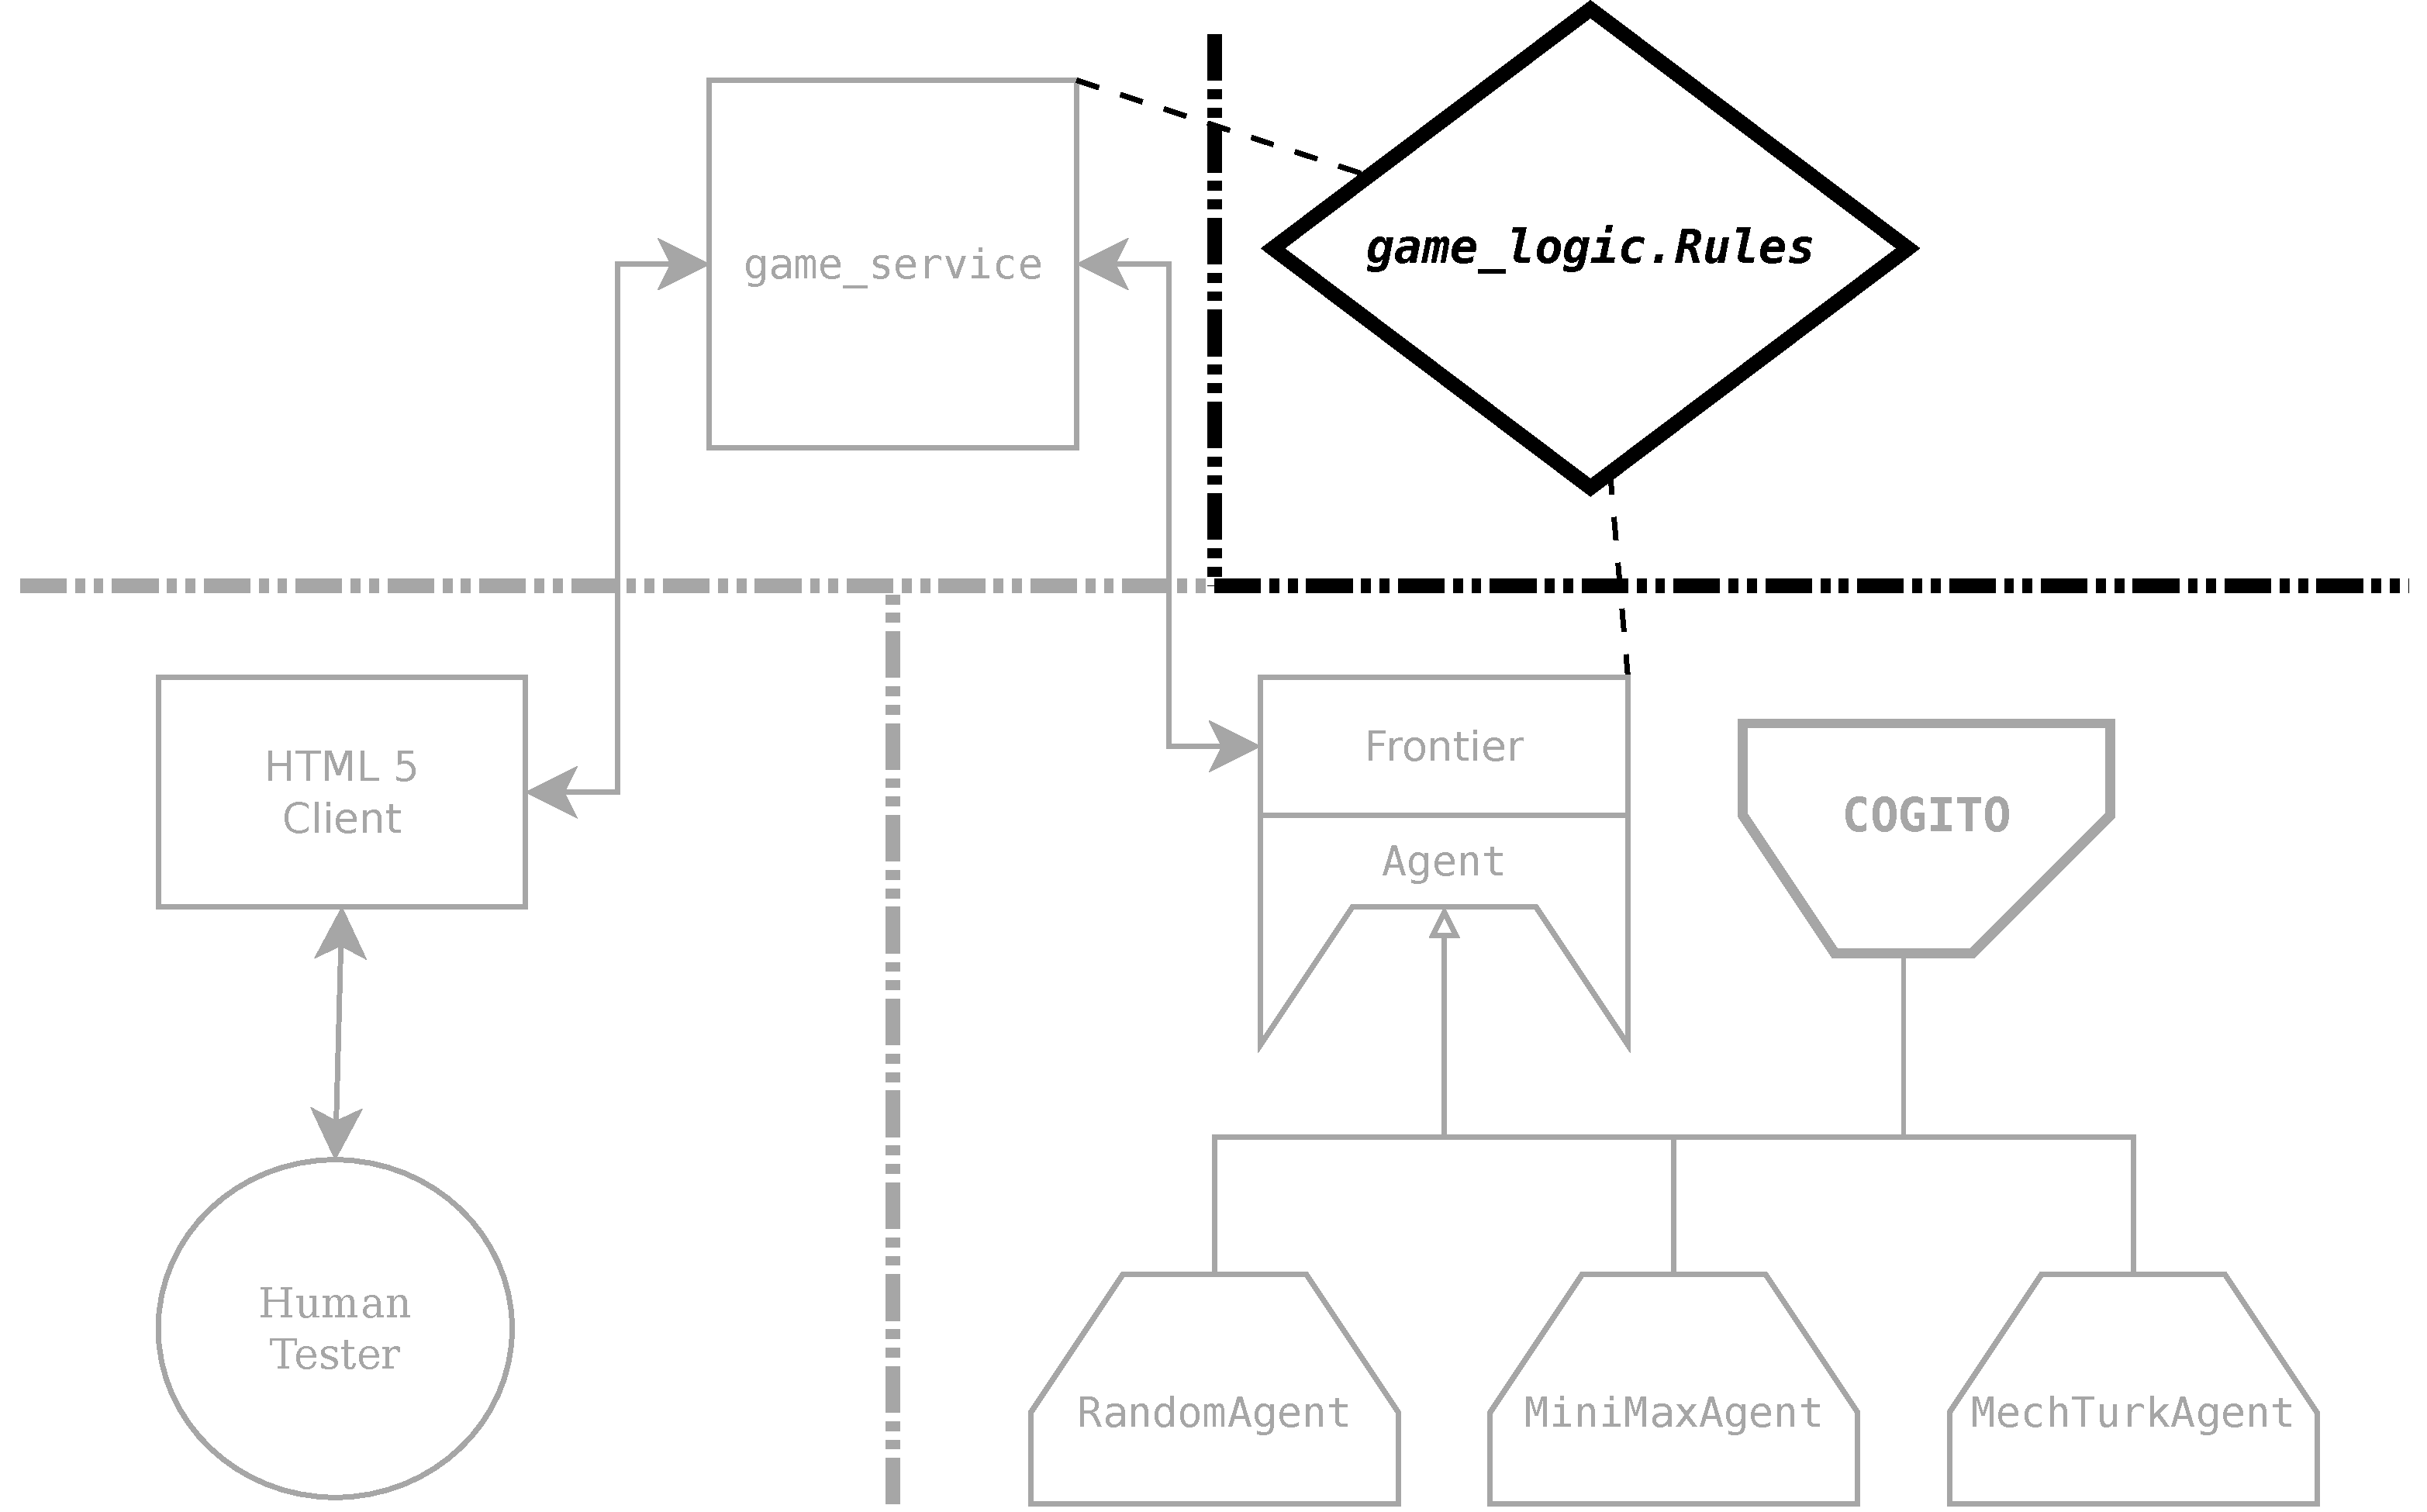
\includegraphics[width=\textwidth]{files/william/archi_lib} 
\caption{Rôle de \texttt{\gls{game_logic}} dans le système.} 
\end{figure}

Nous avons également parlé dans le chapitre~\ref{section_analyse_environnement} d'un agent \og Arbitre \fg{} maître du jeu qui a besoin d'un ensemble de règles afin d'initialiser le plateau et d'appliquer ou de refuser respectivement les coups légaux et illégaux.

Il est claire que ces deux objets partagent un même ensemble de fonctions et de structures. Nous avons donc fait le choix de les factoriser dans une bibliothèque que nous appellerons \texttt{game\_logic}.
\begin{figure}[H] 
\centering
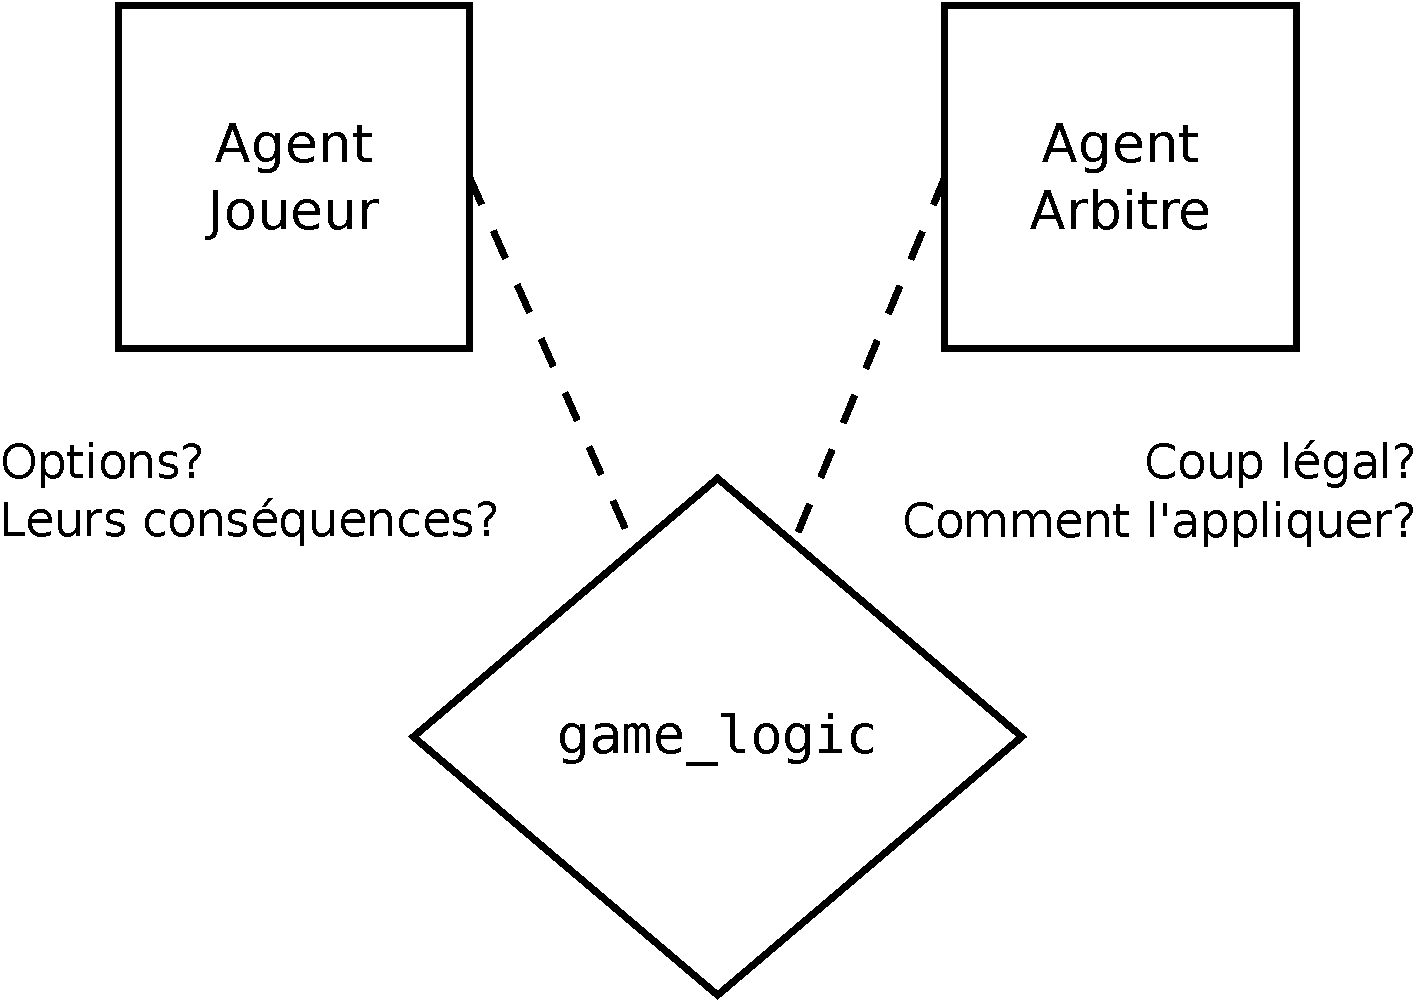
\includegraphics[width=0.75\textwidth]{files/env/game_logic_shared} 
\caption{Partage de la bibliothèque \texttt{game\_logic}.} 
\label{game_logic_shared}
\end{figure}
Cette bibliothèque contient trois classes principales :
\begin{itemize}
\item \texttt{BoardMatrix} : plateau sous forme matricielle avec accesseurs adaptés,
\item \texttt{Rules} : interface implémentée par chaque jeu. Ses méthodes permettent de connaître :
\begin{itemize}
\item la forme du plateau et sa configuration initiale,
\item qui joue en premier,
\item quand la partie est gagnée ou perdue et par qui, quand le match est nul,
\item les coups possibles pour un joueur donné.
\end{itemize}
\item \texttt{Game} : associe un objet \texttt{Rules}, un objet \texttt{BoardMatrix}, un état et un joueur courant.
\end{itemize}
\begin{figure}[H] 
\centering
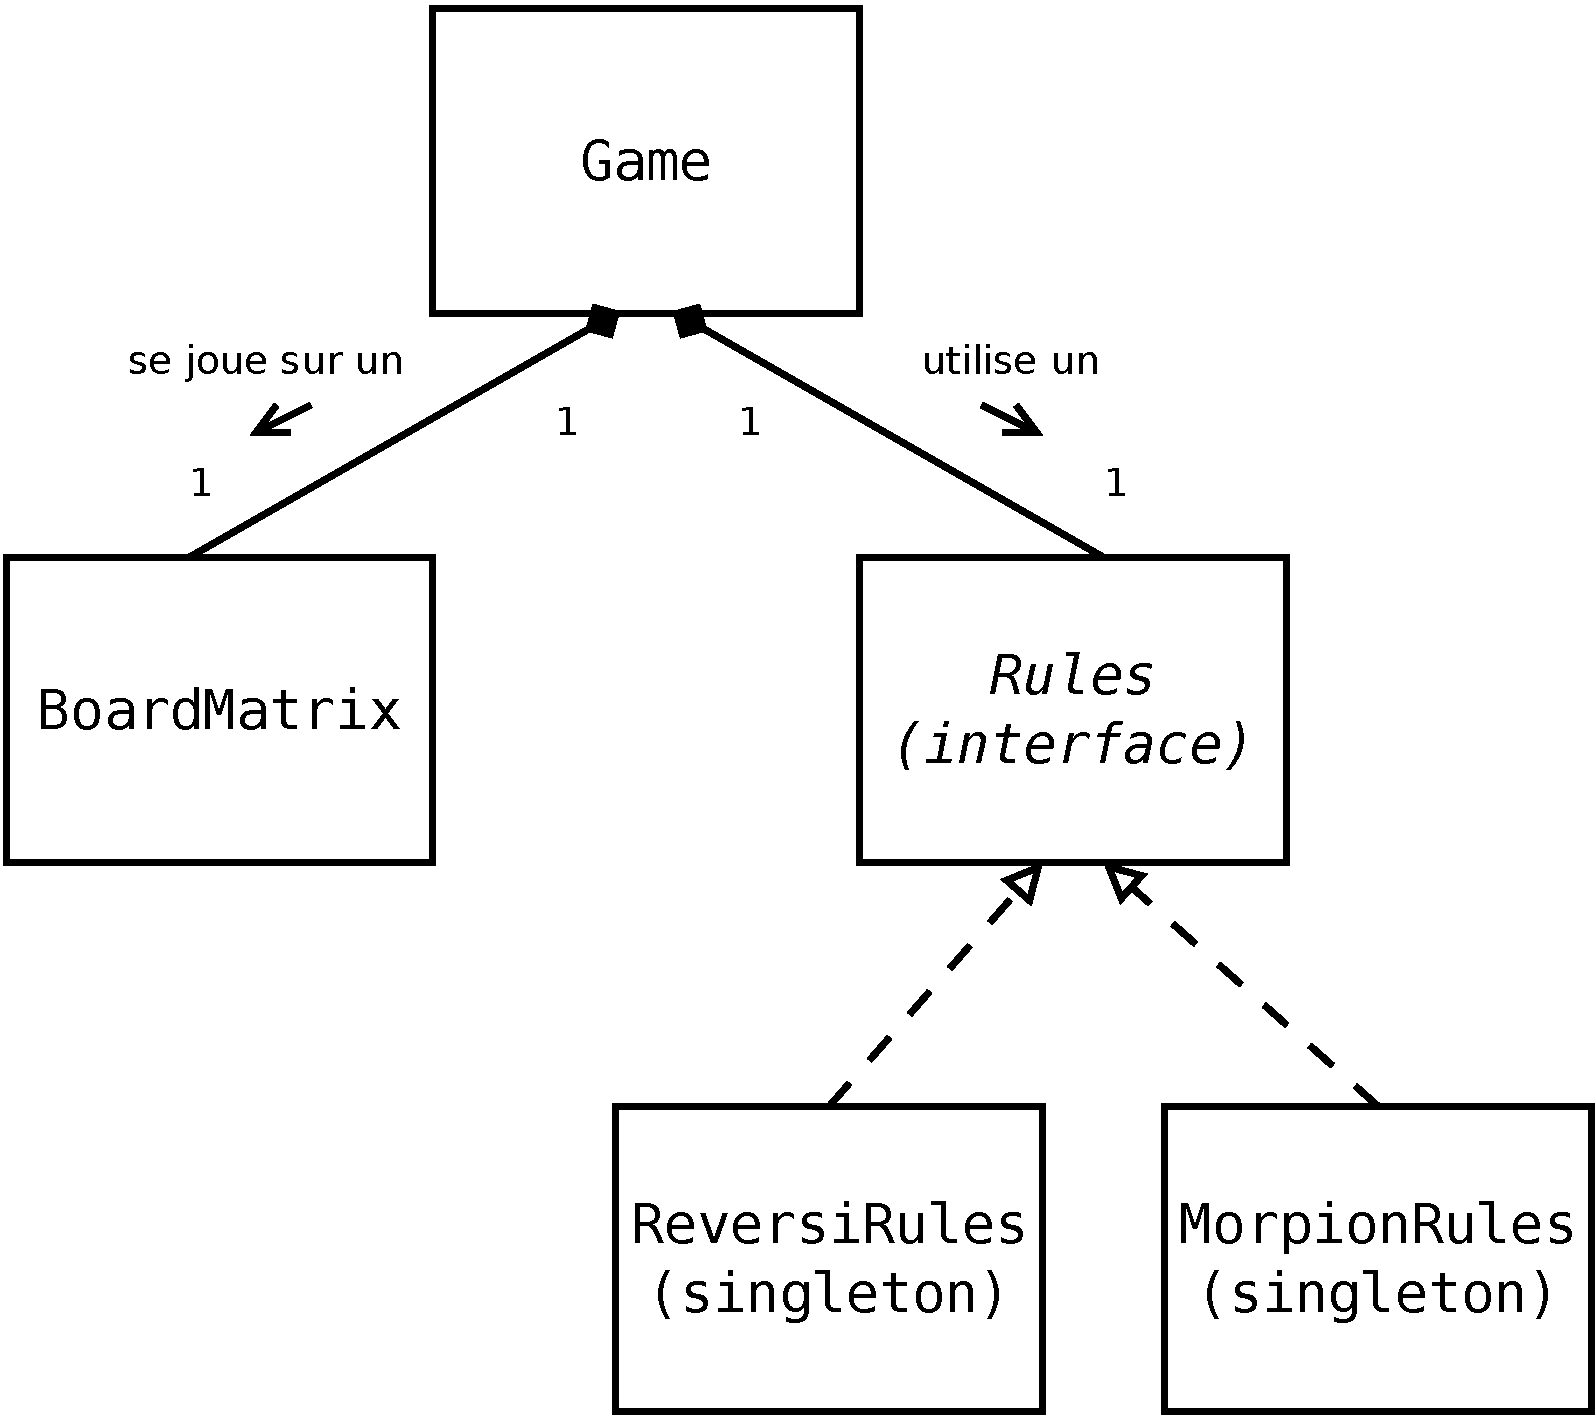
\includegraphics[width=0.75\textwidth]{files/env/game_logic} 
\caption{Classes de la bibliothèque \texttt{game\_logic}.} 
\label{game_logic}
\end{figure}

%---------------------------------------------------------------------------------------------------
% GAME SERVICE
%---------------------------------------------------------------------------------------------------
\subsection{Serveur \texttt{game\_service}}
Le chapitre~\ref{section_analyse_environnement} conclu en proposant le modèle client-serveur pour les communications entre l'\emph{agent-joueur} et l'\emph{agent-arbitre}.

\begin{figure}[H] 
\centering
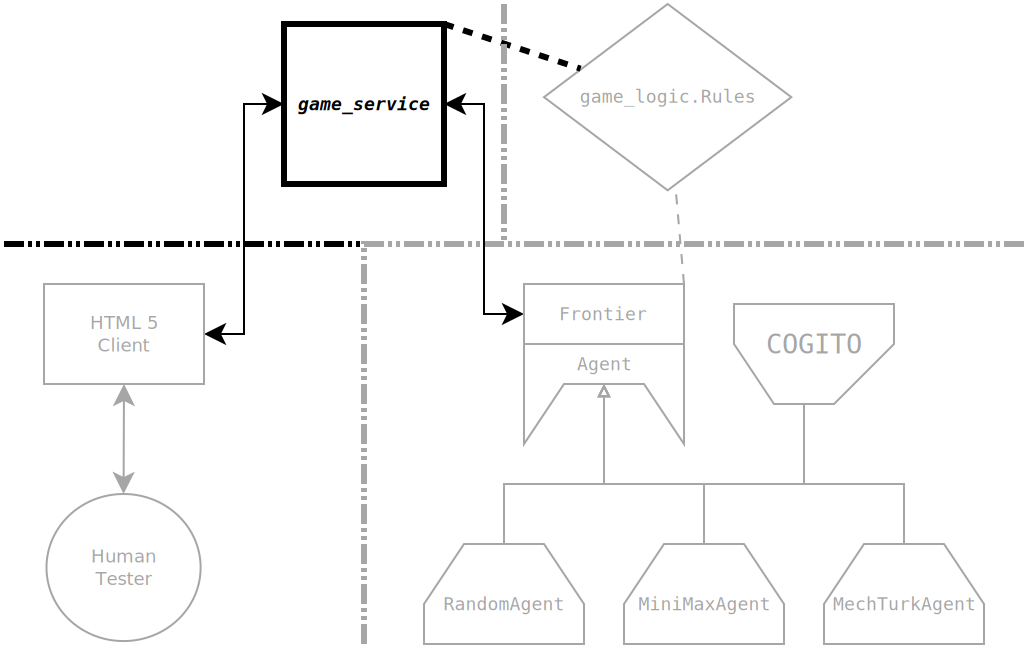
\includegraphics[width=\textwidth]{files/william/archi_serveur} 
\caption{Rôle de \texttt{game\_service} dans le système.} 
\end{figure}

L'arbitre et l'environnement, c'est à dire l'état du jeu, seront hébergés dans une application à part entière : un \og web service \fg{} appelé \texttt{game\_service}.
\subsubsection{Transfert des percepts}
Le client-joueur a tout d'abord besoin de percevoir son environnement, c'est à dire de connaître l'état courant du jeu. Il est envoyé par le serveur sous forme d'un  document \texttt{XML}\footnote{ XML : Extensible markup language. } grâce au protocole \texttt{HTTP}\footnote{ HTTP : Hyper-text transfer  protocol. }. Pilier du web, l'\texttt{HTTP} a l'avantage d'être très  répandu, ubiquité qui assure l'existence de bibliothèques ouvertes,  complètes, bien documentées et simples d'utilisation pour tous langages et plateformes. Ce choix nous a permit de faciliter le développement du serveur indépendamment du reste du système.
\subsubsection{Transfert des actions}
Le client a également besoin d'envoyer ses coups au serveur. Pour ceci il suffit de paramétrer la requête pour indiquer :
\begin{itemize}
\item celui qui joue,
\item une ligne,
\item une colonne.
\end{itemize}
Il nous est désormais possible d'interagir avec le serveur en écrivant manuellement nos coups dans la barre d'adresse et en lisant le document XML renvoyé. Cette manière de jouer est peu ergonomique, mais elle nous a permis de tester le fonctionnement du serveur en son intégralité bien avant la construction d'une interface graphique.

À noter également qu'il n'y a pas d'authentification ou de gestion des utilisateurs. Il est donc possible de \og tricher \fg{} en prenant le tour de l'autre joueur  : nous supposons ici qu'il n'y a simplement pas de tricheur. Nous avons choisi d'ignorer ces problèmes de sécurité dans le but de se concentrer sur d'autres parties du système plus en rapport avec notre sujet. Il serait cependant simple d'ajouter une identification via des sessions et des cookies.
\subsubsection{Constitution des réponses}
Pour analyser ces requêtes paramétrées et générer une réponse, la technologie \og Java Servlet \fg {} est utilisée. Une classe Java est instanciée par un serveur \emph{Tomcat} pour traiter une seule requête : l'objet est détruit immédiatement après avoir envoyé sa réponse sous la forme d'un document XML.

Cette technologie orientée prototypage rapide est très simple à utiliser mais nous permet pourtant de gérer de multiples requêtes concurrentes, donc lancer un très grand nombre de jeux entre différentes paires de clients. Il suffit d'ajouter un paramètre à la requête pour préciser l'identificateur du jeu, et un singleton côté serveur pour stoker les jeux et gérer les accès concurrents.
\subsubsection{Conclusion}
Le serveur correspond finalement un service web, c'est à dire un programme fournissant des données destinées à être lues par des autres programmes et non des humains.
\begin{figure}[H] 
\centering
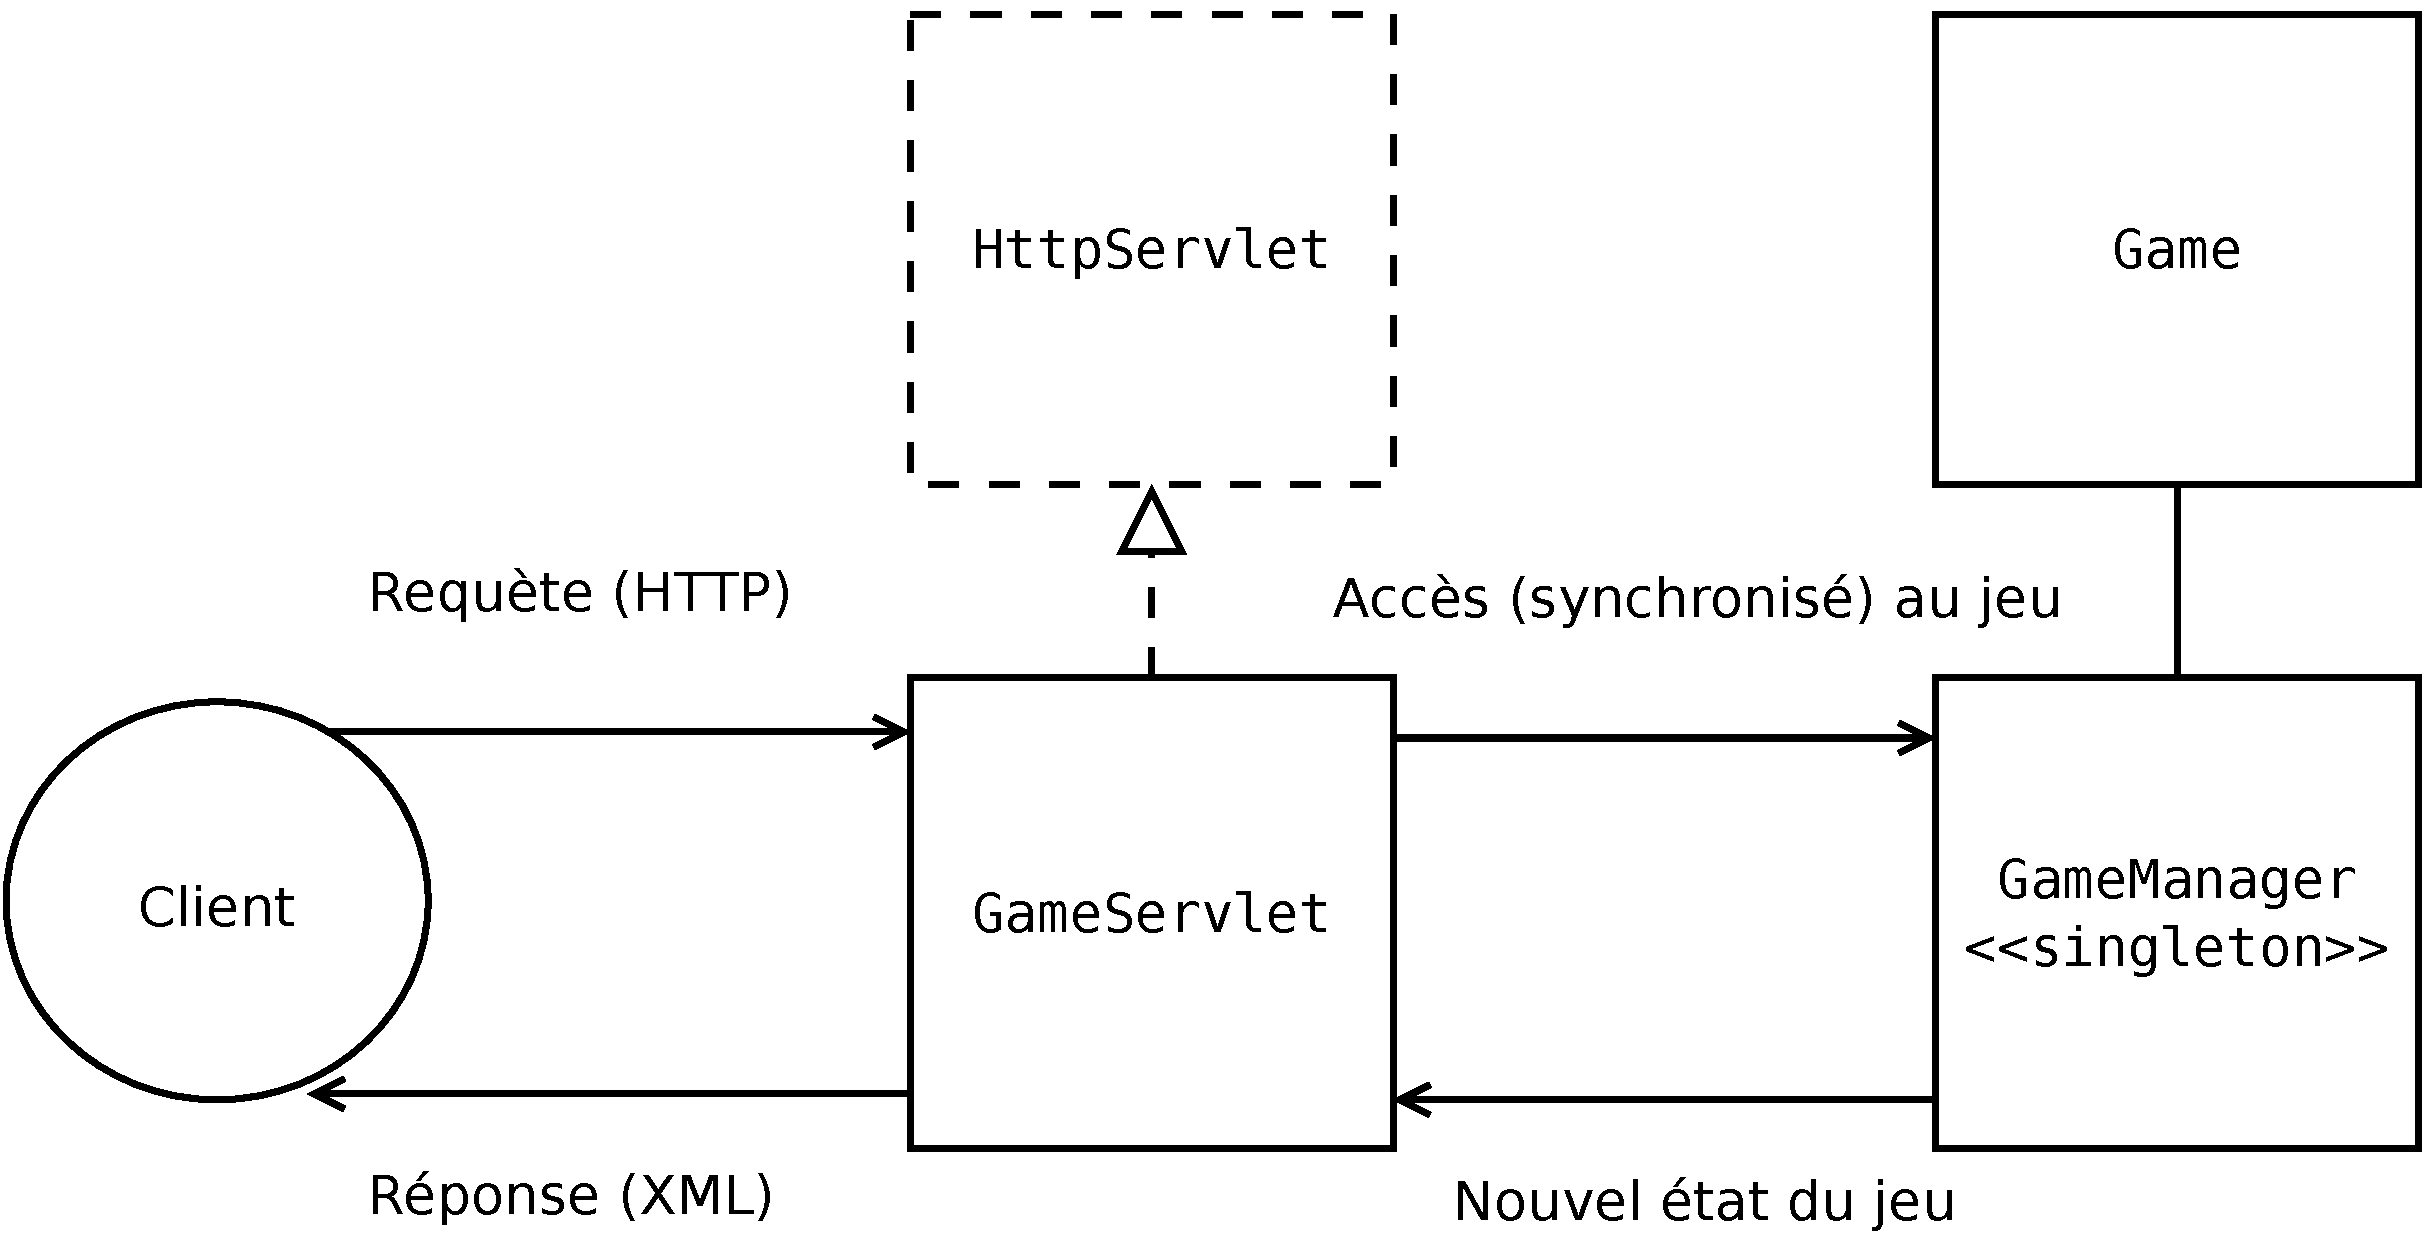
\includegraphics[width=\textwidth]{files/env/game_service} 
\caption{Classes du Service Web \texttt{game\_service}.} 
\label{game_service}
\end{figure}
Le \texttt{GameManager} sert de base de données temporaire : c'est un conteneur de \texttt{Game}, classe de la bibliothèque \texttt{game\_logic}. Chaque \texttt{Game} possédant une référence vers le singleton \texttt{Rules}, il est possible pour le serveur d'arbitrer tous les parties simultanément.

%---------------------------------------------------------------------------------------------------
% CLIENTS
%---------------------------------------------------------------------------------------------------
\subsection{Clients}
%---------------------------------------------------------------------------------------------------
% CLIENT HUMAIN
%---------------------------------------------------------------------------------------------------

\subsubsection{Client humain}
Le client humain est notre plateforme de visualisation des performances de \cogito{}.

\begin{figure}[H] 
\centering
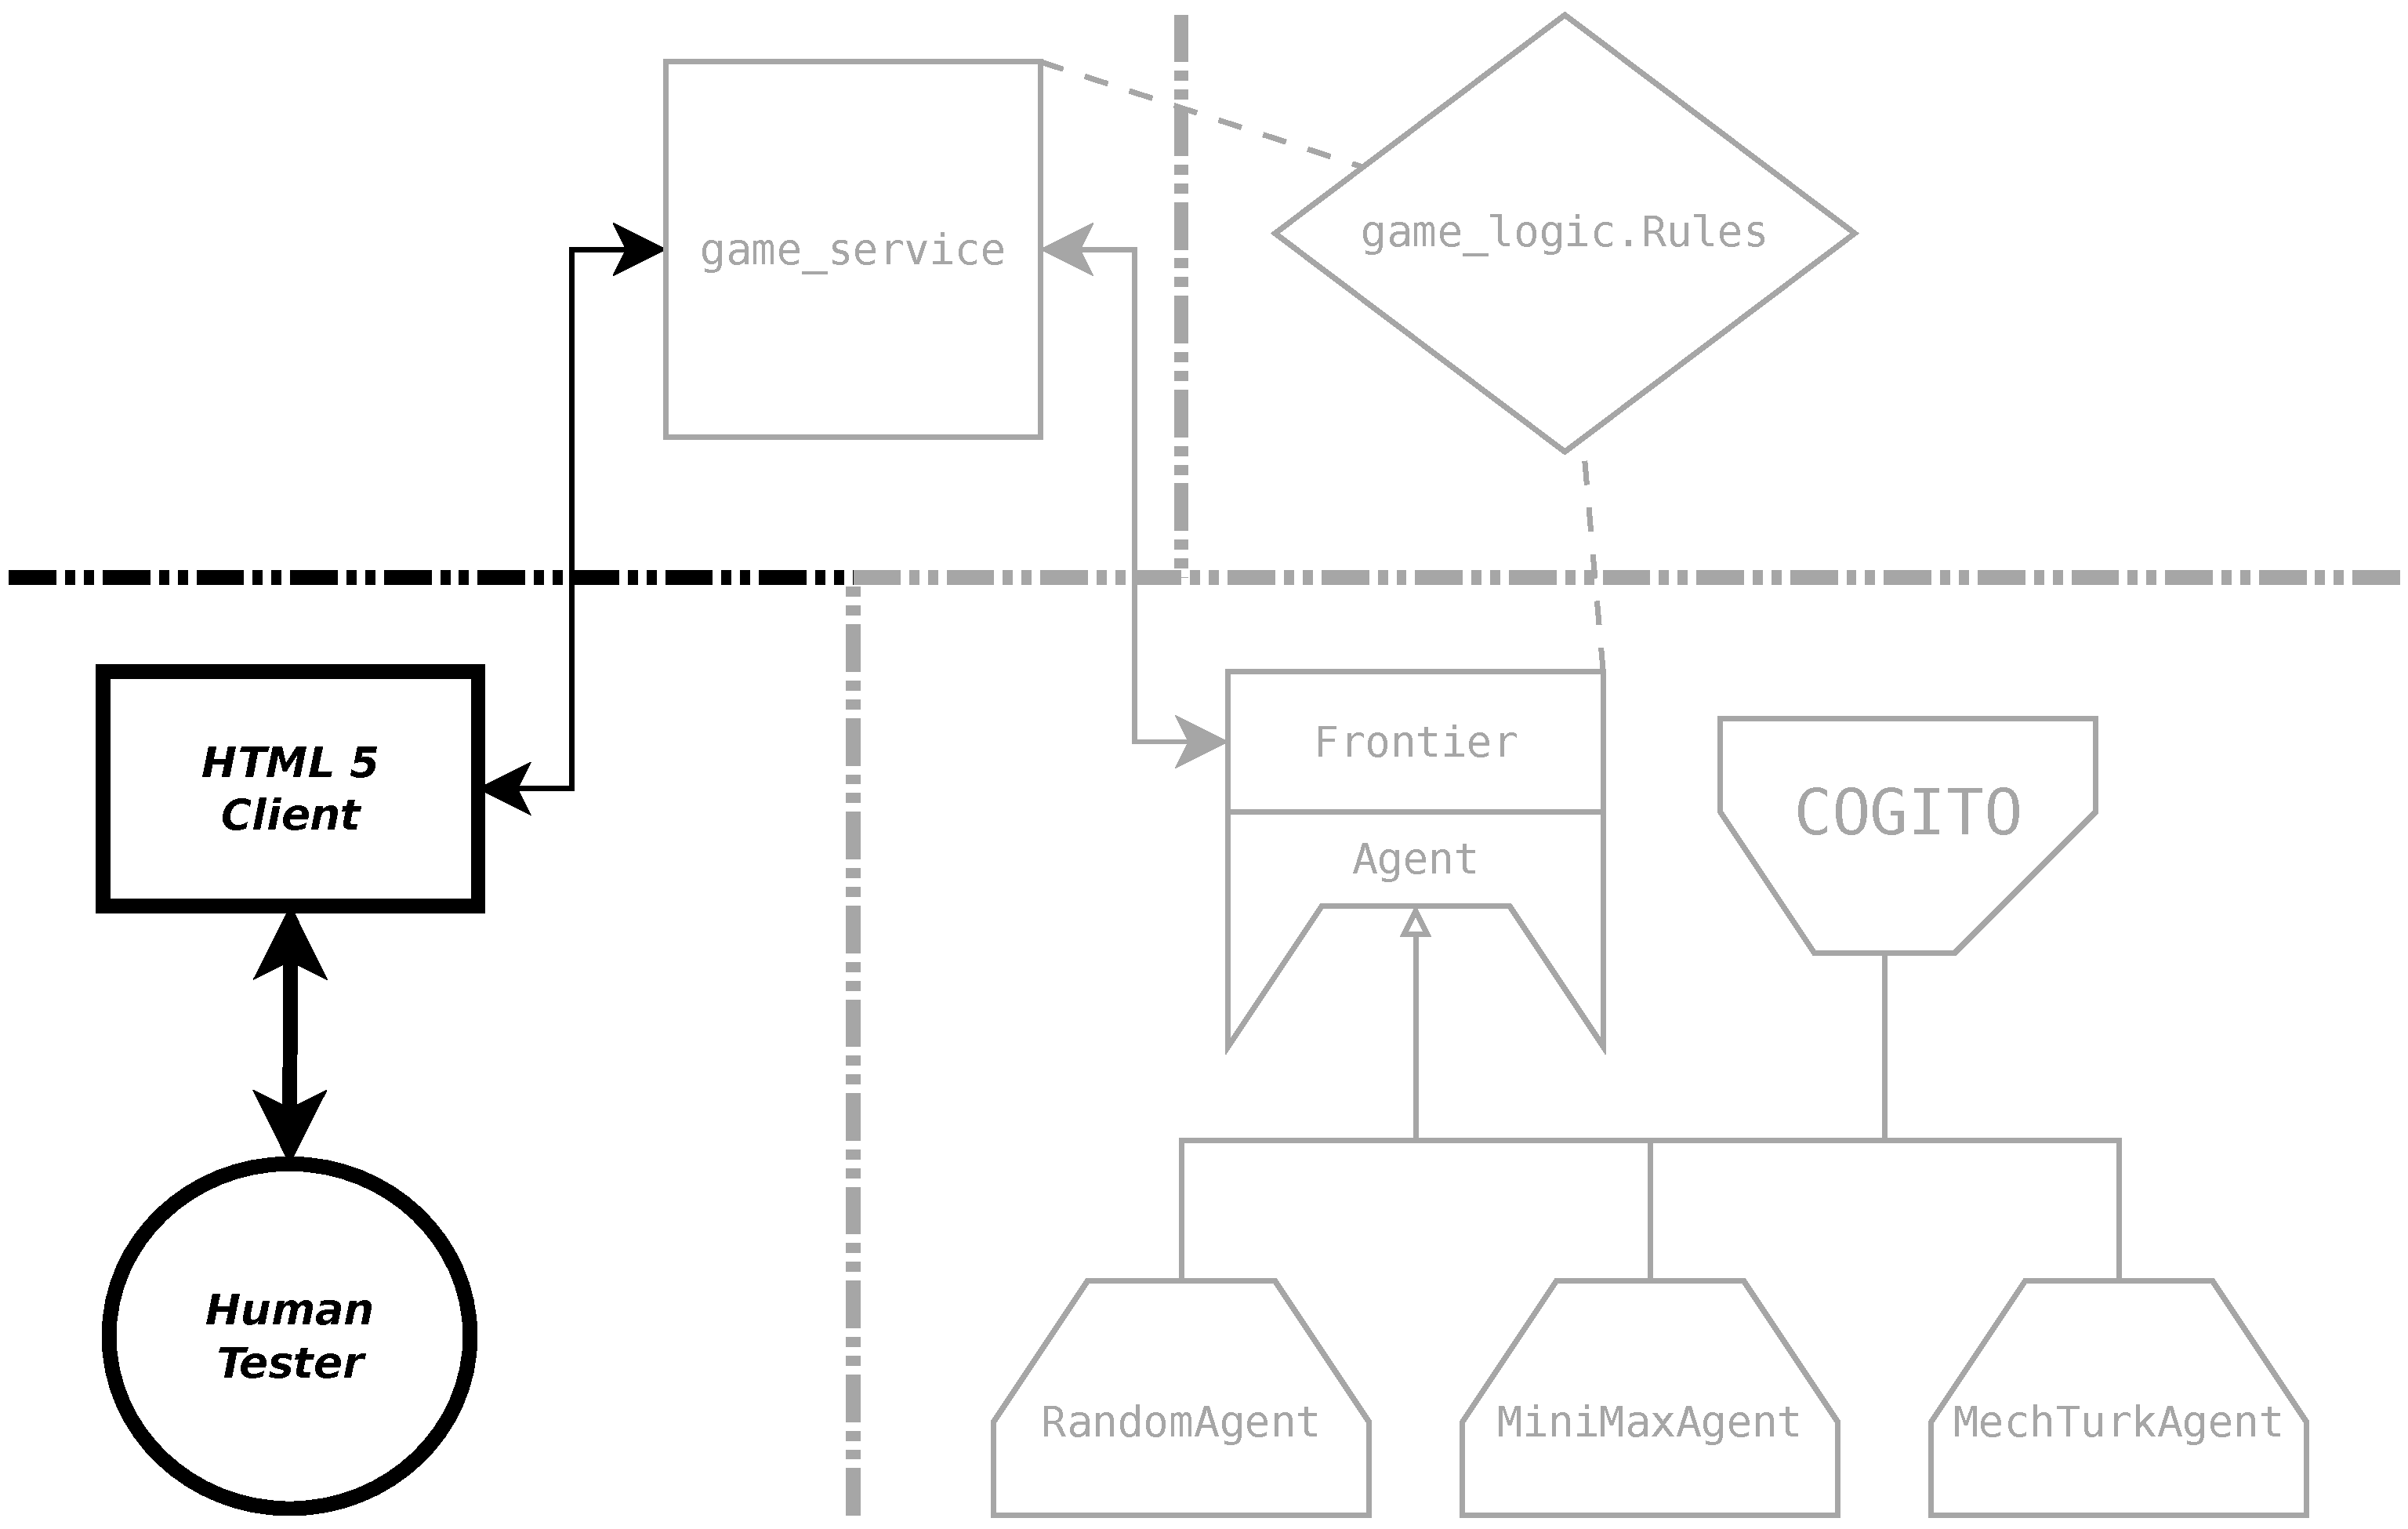
\includegraphics[width=\textwidth]{files/william/archi_client_humain} 
\caption{Rôle du client humain dans le système.} 
\end{figure} 

L'homme se repose sur sa vision pour comprendre le monde.Posséder une sortie graphique prototypique au début du développement a facilité le développent et le débogage. L'\texttt{HTML 5} a comme avantage d'être un standard multi-plateforme et non-compilé. Seul un navigateur web récent est nécessaire.

\og \texttt{HTML 5} \fg{} est plus qu'un ensemble de balises \texttt{HTML}. Il s'agit surtout d'une bibliothèque \texttt{javascript}, étant conçu pour parcourir et manipuler le \texttt{DOM}\footnote{DOM : Document Object Model.}. Couplé avec la technologie \texttt{AJAX}\footnote{AJAX : acronyme d'Asynchronous Javascript and XML.} nous pouvons facilement interagir avec notre serveur via des requêtes \texttt{HTTP} formatées en \texttt{XML}.

Tout ceci nous permet, encore une fois, d'éviter le développent d'infrastructure peu intéressant en utilisant des technologies Libres, standardisé et couramment utilisés.   

%---------------------------------------------------------------------------------------------------
% CLIENT MACHINE
%---------------------------------------------------------------------------------------------------
\subsubsection{Client machine}

\begin{figure}[H] 
\centering
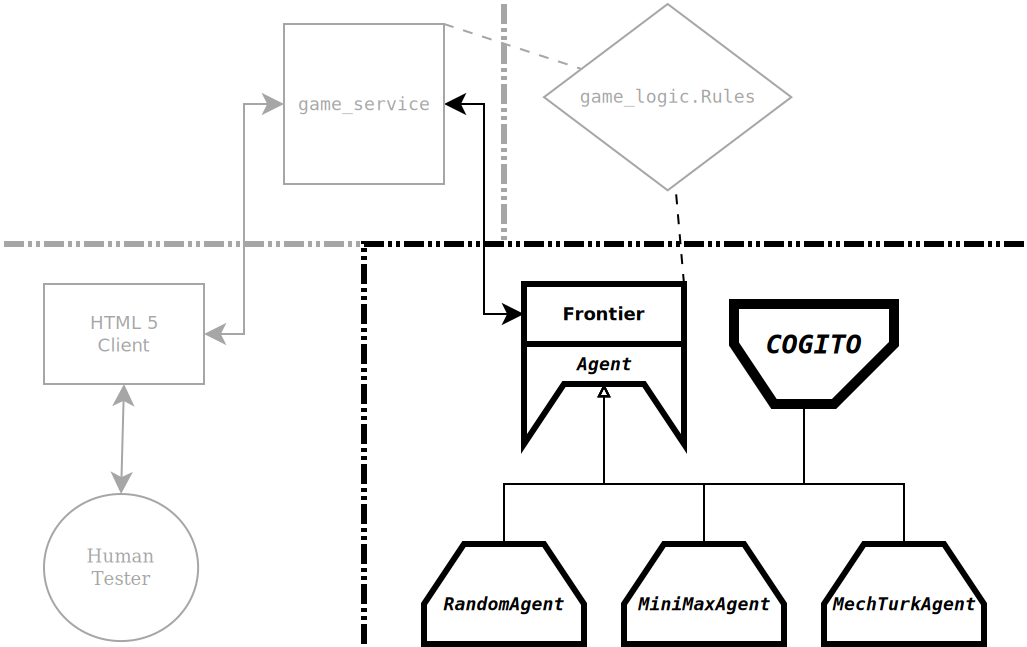
\includegraphics[width=\textwidth]{files/william/archi_client_machine} 
\caption{Rôle de l'agent-client dans le système.} 
\end{figure}

\subsubsection{Classe \texttt{Frontier}}
La frontière est une module purement réactif composé d'un \texttt{Actuator}, traduisant les objets \texttt{Action} qu'il reçoit en requêtes \texttt{HTTP}, et d'un \texttt{Sensor}, qui transforme les réponses \texttt{XML} en objets \texttt{Percept} dont le plus important est le percept \texttt{Choices}.

En claire ce sont des traducteurs : le \texttt{Sensor} traduit du langage \texttt{Agent} au langage arbitre, l' \texttt{Actuator} l'inverse. La \texttt{Frontier} comporte aussi une sorte de mémoire sensorielle lui permettant de juger si son environnement ait changé. Nous ne passons donc que les percept intéressantes aux couches plus hautes dans l'hiérarchie.  

\subsubsection{Classe abstraite \texttt{Agent}}
Un \texttt{Frontier} est toujours encapsulé par un \texttt{Agent} et sert d'outil pour celui-ci. Cette classe \texttt{Agent} est instancié au démarrage du client machine : le fil d'exécution principale boucle à l'intérieure de celui-ci pour alterner entre demandes de mises à jour du serveur, réflexion et choix de coup. C'est une classe purement abstraite, car l'implémentation de ces deux dernières fonctionnalités varie énormément d'un algorithme et un autre. Parmi nos agents-paramètres se trouvent :
\begin{itemize}
\item \texttt{MiniMaxAgent} qui applique la stratégie de maximisation de gain minimale. 
\item \texttt{RandomAgent} qui génère de nombres aléatoires pour choix au hasard ses coups.
\item \texttt{MechTurkAgent} qui pour des raisons que nous ignorons exhibe une intelligence quasi-humaine\footnote{nous vous taquinons : en vrai c'est à l'utilisateur de choisir ses coups avec la console. }.
\item \texttt{Cogito} notre cognition artificielle qui apprend à jouer en jouant contre les autres.
\end{itemize}
Notons que rien d'empêche les confrontations entre deux clients machines avec des IA différents, un client humain et un client machine ou bien deux clients humains. Par la suite nous nous focaliserons entièrement sur l'implémentation de ce dernière : tout cette architecture fut, d'après tout, posons que pour lui.